\section*{課題1}
多クラス(2クラス以上)のサンプル(2次元以上とする)を,各クラスに対して設定した正規分布などに基づく乱数の発生により生成した後,一部を学習サンプル,残りをテストサンプルとし,学習サンプルを用いて学習した識別器を用いてテストサンプルを分類するプログラムを作成せよ.

\subsection*{サンプル生成方法}
本実験ではサンプルとして,2クラスの2次元正規分布に基づくデータを作成した.
手法としては1次元の正規分布データの作成を各基底において行うという非常にシンプルなものである.

\subsection*{設定条件}
今回は2種類の設定によるデータセットで実験を行った.
\begin{itemize}
    \setlength{\itemsep}{3mm}
    \item データセットA\par
    \quad
    クラス1は平均5,分散2.5の2次元正規分布,クラス2は平均-5,分散2.5の2次元正規分布に基づくデータの集合.
    \item データセットB\par
    \quad
    クラス1は平均3,分散2.5の2次元正規分布,クラス2は平均-3,分散2.5の2次元正規分布に基づくデータの集合.
\end{itemize}

\subsection*{実験結果}
各データセットに対する識別結果は以下のようになった.
\begin{figure}[H]
    \begin{minipage}{0.5\hsize}
        \begin{center}
            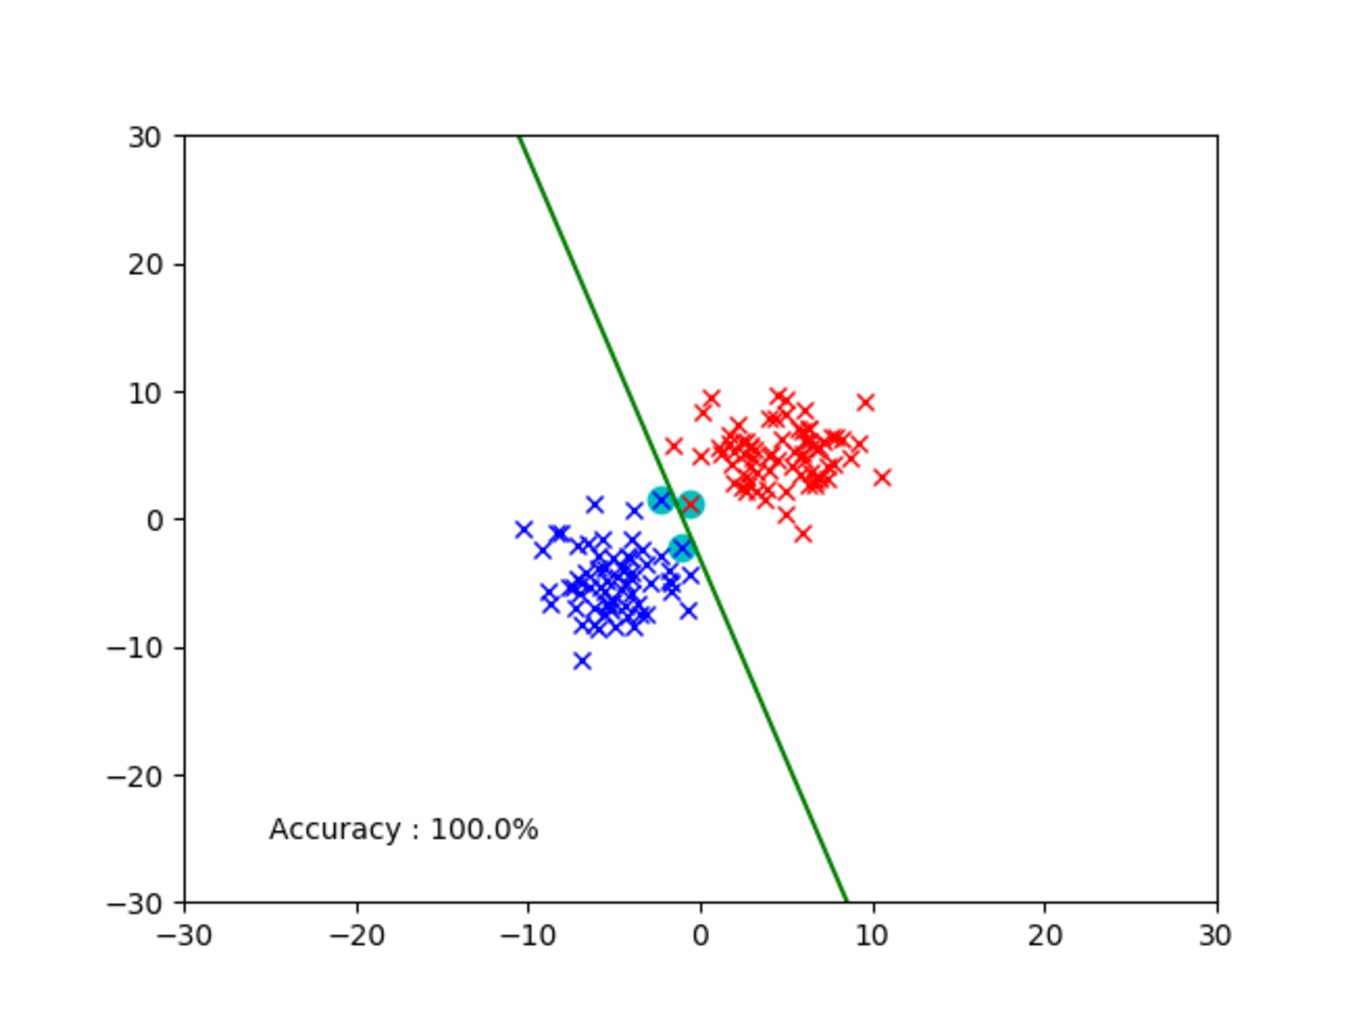
\includegraphics[width=75mm]{./figures/task1/Figure_200_train.eps}
        \end{center}
    \end{minipage}
    \begin{minipage}{0.5\hsize}
        \begin{center}
            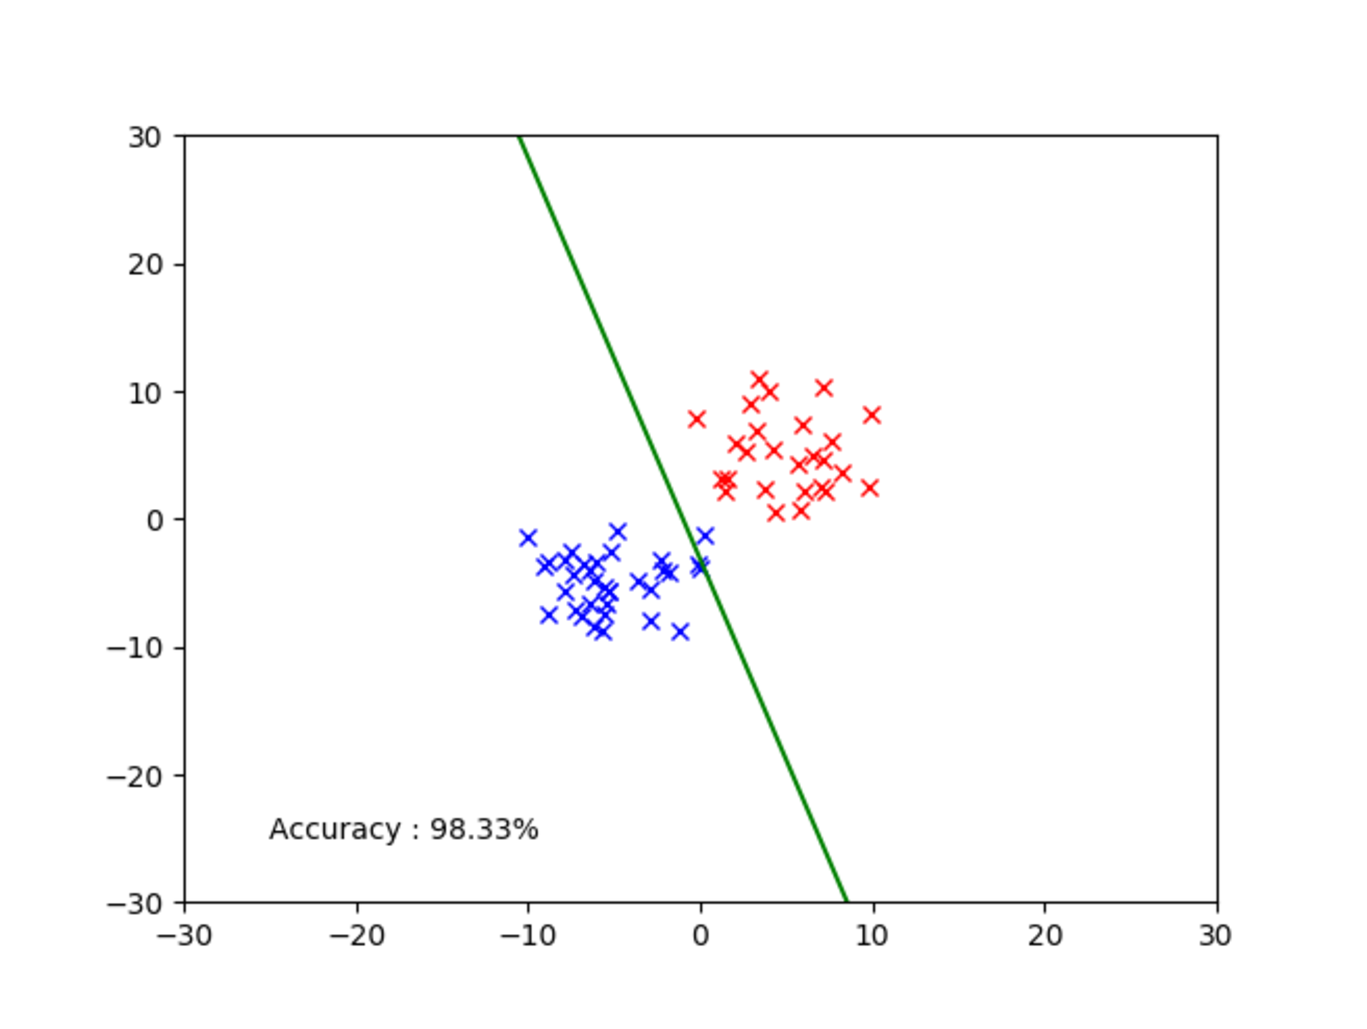
\includegraphics[width=75mm]{./figures/task1/Figure_200_test.eps}
        \end{center}
    \end{minipage}
    \caption{SVMによるデータセットAに対する識別結果(左:トレーニングデータ 140個,右:テストデータ 60個)}
    \label{graph1}
\end{figure}
\begin{figure}[H]
    \begin{minipage}{0.5\hsize}
        \begin{center}
            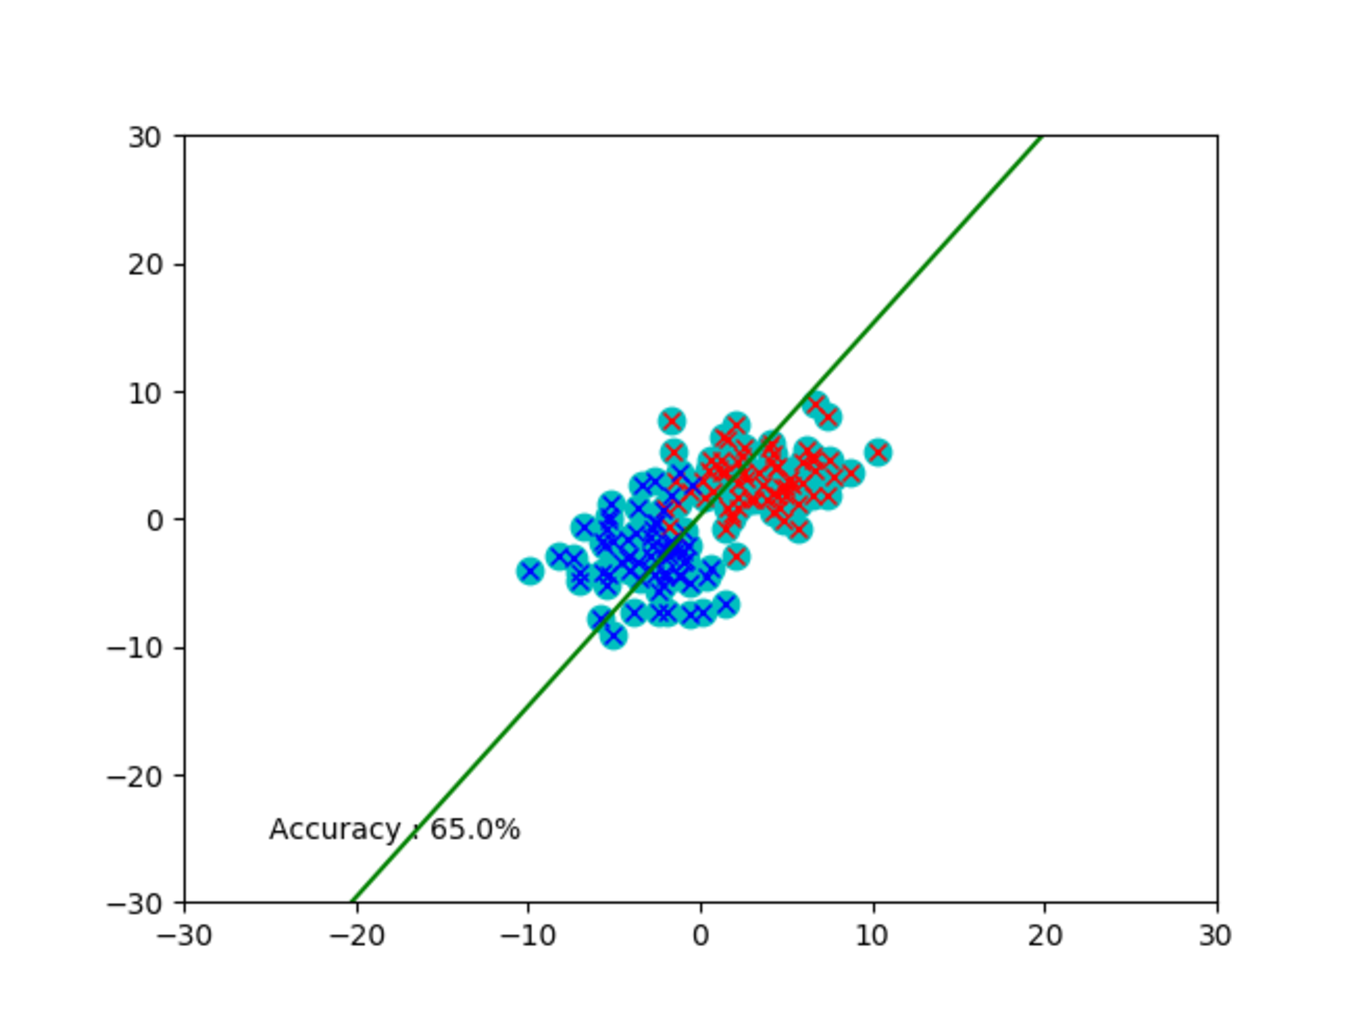
\includegraphics[width=75mm]{./figures/task1/Figure_200_train_fail.eps}
        \end{center}
    \end{minipage}
    \begin{minipage}{0.5\hsize}
        \begin{center}
            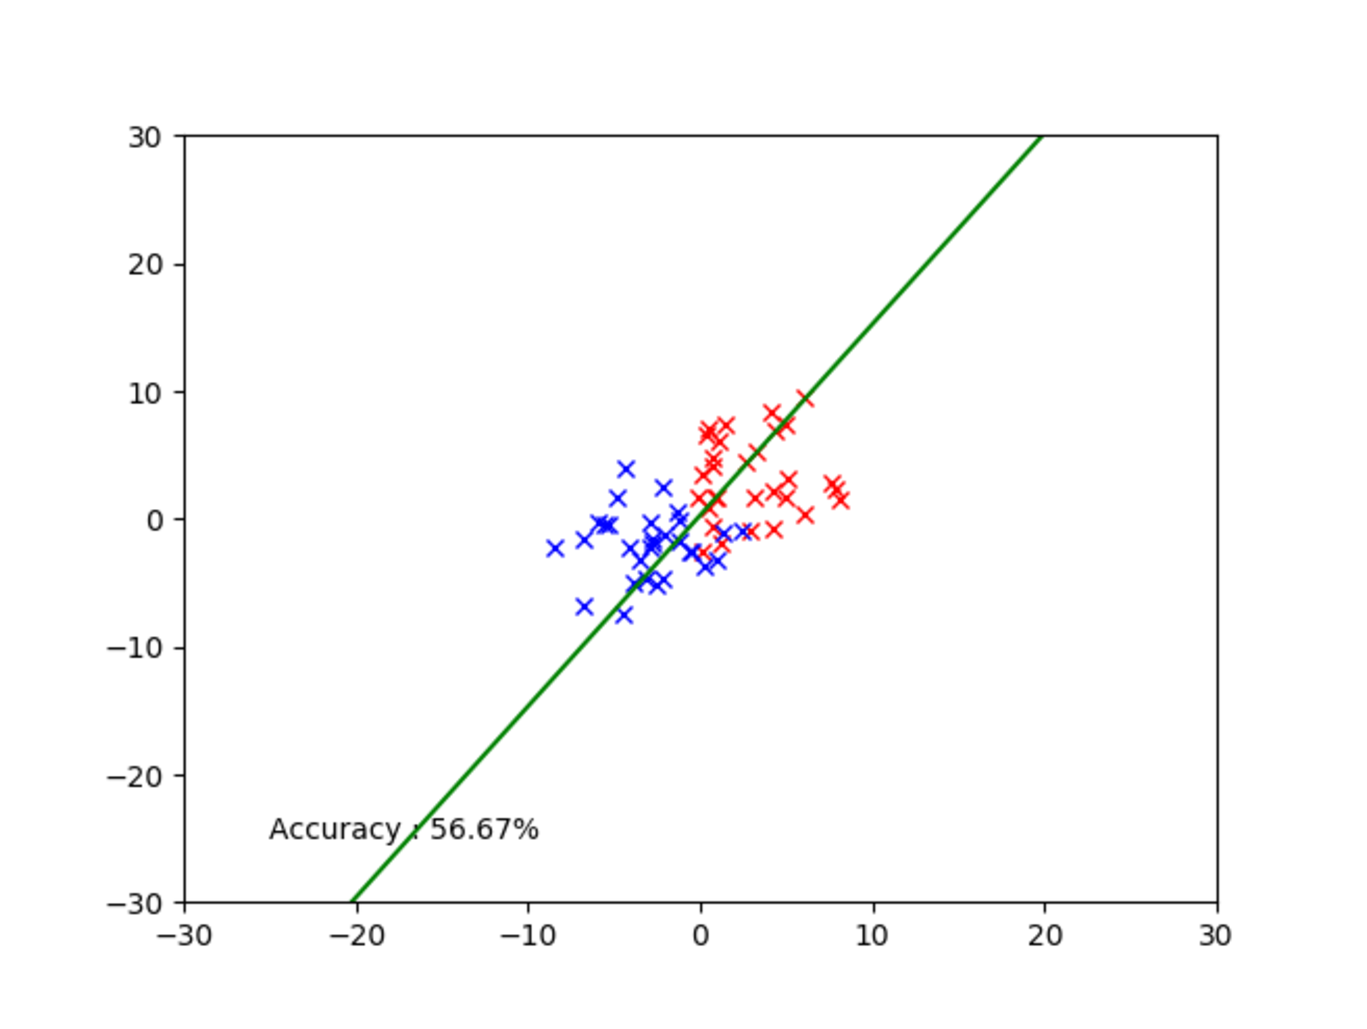
\includegraphics[width=75mm]{./figures/task1/Figure_200_test_fail.eps}
        \end{center}
    \end{minipage}
    \caption{SVMによるデータセットBに対する識別結果(左:トレーニングデータ 140個,右:テストデータ 60個)}
    \label{graph2}
\end{figure}

\subsection*{考察}
実験設定から分かる通り,データセットBはデータセットAに比べてクラス間の距離がなく,重複している.
前述した通り,今回実装したSVMはハードマージンSVMであるので,データセットBに対する識別は厳しいと予想した.\par
まずデータセットAに対する識別結果であるが,図\ref{graph1}から分かるように,ある程度うまく識別されていると言える.\par
続いてデータセットBに対する識別結果であるが,図\ref{graph2}から分かるように,識別精度は非常に低いものとなった.\par
結果としては予想通りなものとなり,ハードマージンSVMが重複のあるデータに非常に弱いことも見て取れる結果となった.